\documentclass[default]{beamer}
\setbeamertemplate{navigation symbols}{}

\usetheme{CambridgeUS}
\useoutertheme{infolines}
%\usecolortheme{crane}

\usepackage{cmap}							% Поддержка поиска русских слов в PDF (pdflatex)
\usepackage[utf8]{inputenc}					% Выбор языка и кодировки
\usepackage[english, russian]{babel}
\usepackage{csquotes}

\usepackage[
	language=auto,
	autolang=other,
	backend=biber,
	style=authortitle,
	sorting=ydnt
]{biblatex}
\addbibresource{aha.bib}
				
\DeclareSourcemap{
	\maps[datatype=bibtex, overwrite]{
		\map{
			\step[fieldset=langid, fieldvalue=english]
			\step[fieldset=doi, null]
			\step[fieldset=issn, null]
			\step[fieldset=isbn, null]
			\step[fieldset=url, null]
			\step[fieldsource=language, fieldset=langid, origfieldval]
		}
	}
}


\graphicspath{{../../images/}} 			% Пути к изображениям

\makeatletter
\setbeamertemplate{footline}
{
	\leavevmode%
	\hbox{%
		\begin{beamercolorbox}[wd=.333333\paperwidth,ht=2.25ex,dp=1ex,center]{author
				in head/foot}%
			\usebeamerfont{author in
				head/foot}\insertshortauthor~~\beamer@ifempty{\insertshortinstitute}{}{(\insertshortinstitute)}
		\end{beamercolorbox}%
		\begin{beamercolorbox}[wd=.333333\paperwidth,ht=2.25ex,dp=1ex,center]{title in
				head/foot}%
			\usebeamerfont{title in head/foot}\insertshorttitle
		\end{beamercolorbox}%
		\begin{beamercolorbox}[wd=.333333\paperwidth,ht=2.25ex,dp=1ex,right]{date in
				head/foot}%
			\usebeamerfont{date in head/foot}\insertshortdate{}\hspace*{2em}
			\insertframenumber{}\hspace*{2ex} 
		\end{beamercolorbox}
	}%
	\vskip0pt%
}


\renewcommand*{\bibfont}{\tiny}
\setlength\bibitemsep{-5pt}

\begin{document}
	
	\title[Cognitome]{Целеполагание и планирование}
	\author[Панов]{Александр Панов}
	\institute[ИСА РАН]{ИСА РАН}
	\date{18 октября 2017~г.} 
	
	\begin{frame}
		\titlepage
	\end{frame}
		
	\begin{frame}
		\frametitle{David W. Aha}
		
		\footnotesize
		\begin{columns}
			\begin{column}{0.8\textwidth}
				\begin{itemize}
					\item Дэвид Аха "--- специалист по искусственному интеллекту, планирование для автономных роботов.
					\item Сотрудник Морского центра прикладных исследований в искусственном интеллекте, Военно-морская исследовательская лаборатория (Navy Center for Applied Research in Artificial Intelligence, Naval Research Laboratory), Вашингтон, США.
					\item \href{https://www.scopus.com/authid/detail.uri?authorId=6701853513}{Scopus}: 149 статей, 5215 цитирований, h-индекс "--- 25.
				\end{itemize}
			\end{column}
			\begin{column}{0.2\textwidth}
				\begin{figure}
					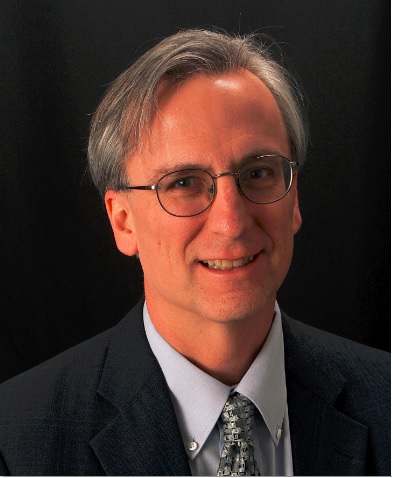
\includegraphics[width=\textwidth]{dwa.jpg}
				\end{figure}
			\end{column}
		\end{columns}
		\par\medskip
		\textbf{Основные публикации:}
		\nocite{*}
		\printbibliography
	\end{frame}

	\begin{frame}
		\frametitle{Мотивация метода целенаправленной автономности (GDA)}
		
		Построенные планы требует модификации в связи с:
		\begin{itemize}
			\item недетерминированностью действий агента,
			\item непредсказуемости окружающей среды (наличие других агентов),
			\item неполнота информации о состояниях среды (область видимости).
		\end{itemize}
	
		Пути решения:
		\begin{itemize}
			\item вероятностное планирование (экспоненциальный рост числа возможных состояний),
			\item адаптивное планирование - с возвратом (перерасход ресурсов),
			\item перепланирование (цели не меняются),
			\item управление множеством целей (GDA).
		\end{itemize}
	\end{frame}

	\begin{frame}
		\frametitle{Концептуальная модель GDA}
		
		\begin{columns}
			\begin{column}{0.6\textwidth}
				\begin{figure}
					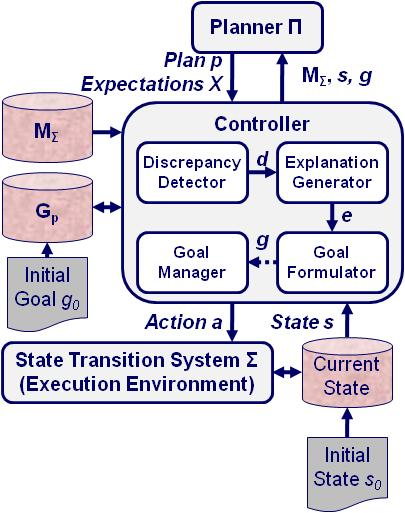
\includegraphics[width=0.8\textwidth]{gda_schema.jpg}
				\end{figure}
			\end{column}
			\begin{column}{0.4\textwidth}
					\begin{itemize}
						\item $M_\Sigma$ - модель среды $\Sigma$, 
						\item $G_p$ - цели в очереди ожидания,
						\item $s$ - текущее состояние,
						\item $g$ - новая цель,
						\item $d$ - расхождение,
						\item $X$ - ожидаемое состояние среды,
						\item $\Pi$ - планировщик (например, SHOP).
					\end{itemize}	
			\end{column}
		\end{columns}
	\end{frame}

	\begin{frame}
		\frametitle{Концептуальная модель GDA}
		
		\begin{columns}
			\begin{column}{0.6\textwidth}
				\begin{figure}
					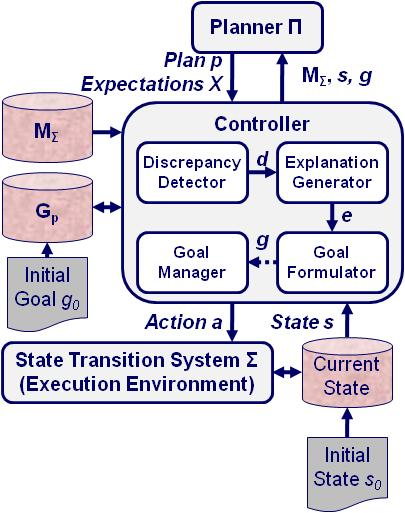
\includegraphics[width=0.8\textwidth]{gda_schema.jpg}
				\end{figure}
			\end{column}
			\begin{column}{0.4\textwidth}
				Основные стадии:
					\begin{enumerate}
						\item Обнаружение рассогласования, непредвиденные события.
						\item Объяснение расхождений.
						\item Формулирование или изменение цели.
						\item Управление множеством целей.
					\end{enumerate}
			\end{column}
		\end{columns}
	\end{frame}
	
	\begin{frame}
		\frametitle{Концептуальная модель GDA}
		
		\begin{columns}
			\begin{column}{0.6\textwidth}
				\begin{figure}
					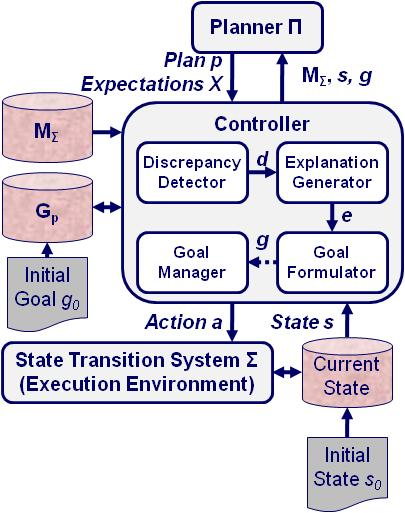
\includegraphics[width=0.8\textwidth]{gda_schema.jpg}
				\end{figure}
			\end{column}
			\begin{column}{0.4\textwidth}
					\begin{enumerate}
						\item Любое расхождение между ожидаемым в плане состояние среды и наблюдаемым.
						\item Основанный на правилах вывод или прецеденты перепланирования.
						\item Основанный на правилах вывод или прецеденты типа <<расхождение-новая цель>>.
						\item Замена текущей цели на новую.
					\end{enumerate}
			\end{column}
		\end{columns}
	\end{frame}


	\begin{frame}
		\frametitle{Жизненный цикл целей}
		
		\centering		
		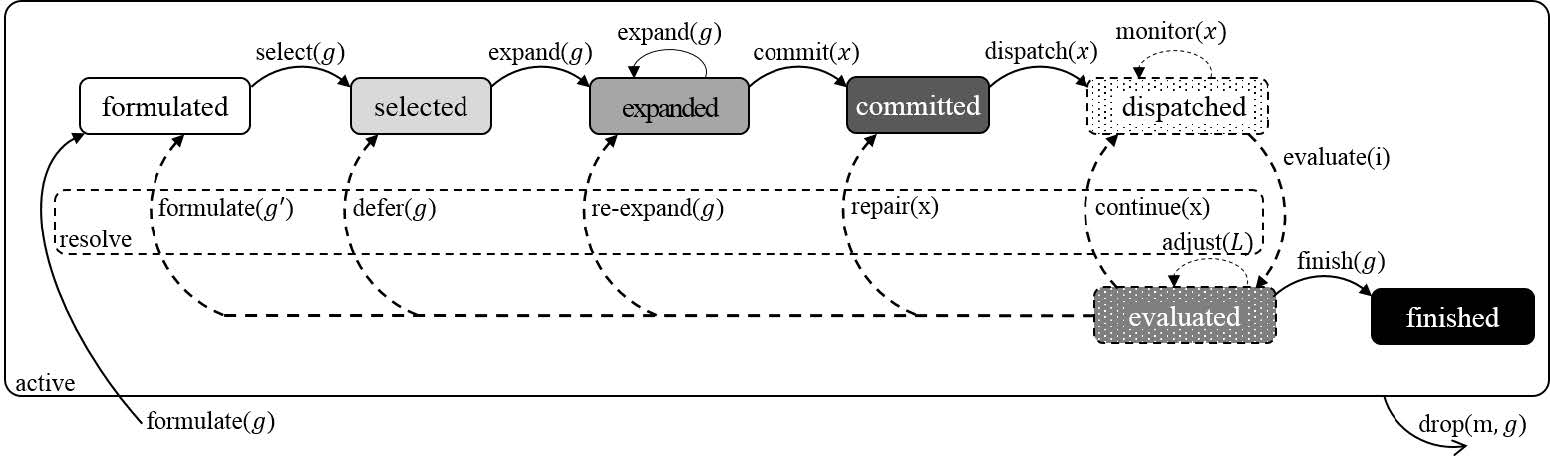
\includegraphics[width=\textwidth]{goal_lifecycle.jpg}
		\begin{itemize}
			\item \textbf{expand} - выделение подцелей и составление плана,
			\item \textbf{dispatch} - выполнение лучшего плана,
			\item \textbf{monitor} - наблюдение за выполнением плана,
			\item \textbf{adjust} - изменение модели среды.
		\end{itemize}
	\end{frame}

	\begin{frame}
		\frametitle{Память целей}
		
		\centering		
		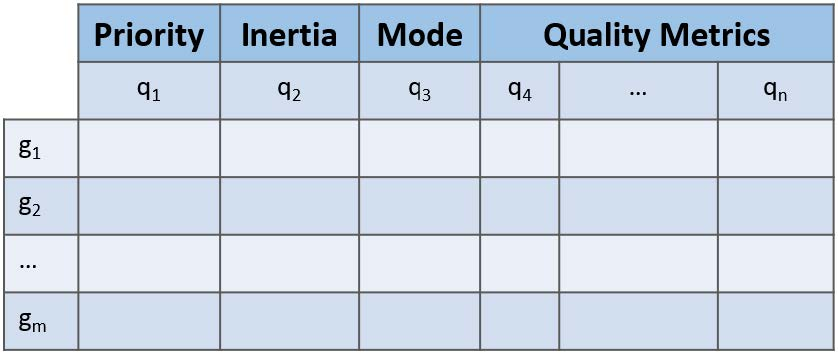
\includegraphics[width=0.5\textwidth]{goal_mem.jpg}
		\par\bigskip
		Задача максимизации общего вознаграждения в случае марковского процесса:
		\[
			V^*(M)=\max_\pi(R(M,\pi)+\gamma\sum_{M'}T(M,\pi,M')V^*(M')),
		\]
		$M$ - состояние памяти целей, $\pi$ - стратегия управления целями, $T$ - функция переходов.
	\end{frame}

	\begin{frame}
		\frametitle{Модельные эксперименты}
		
		\begin{center}
			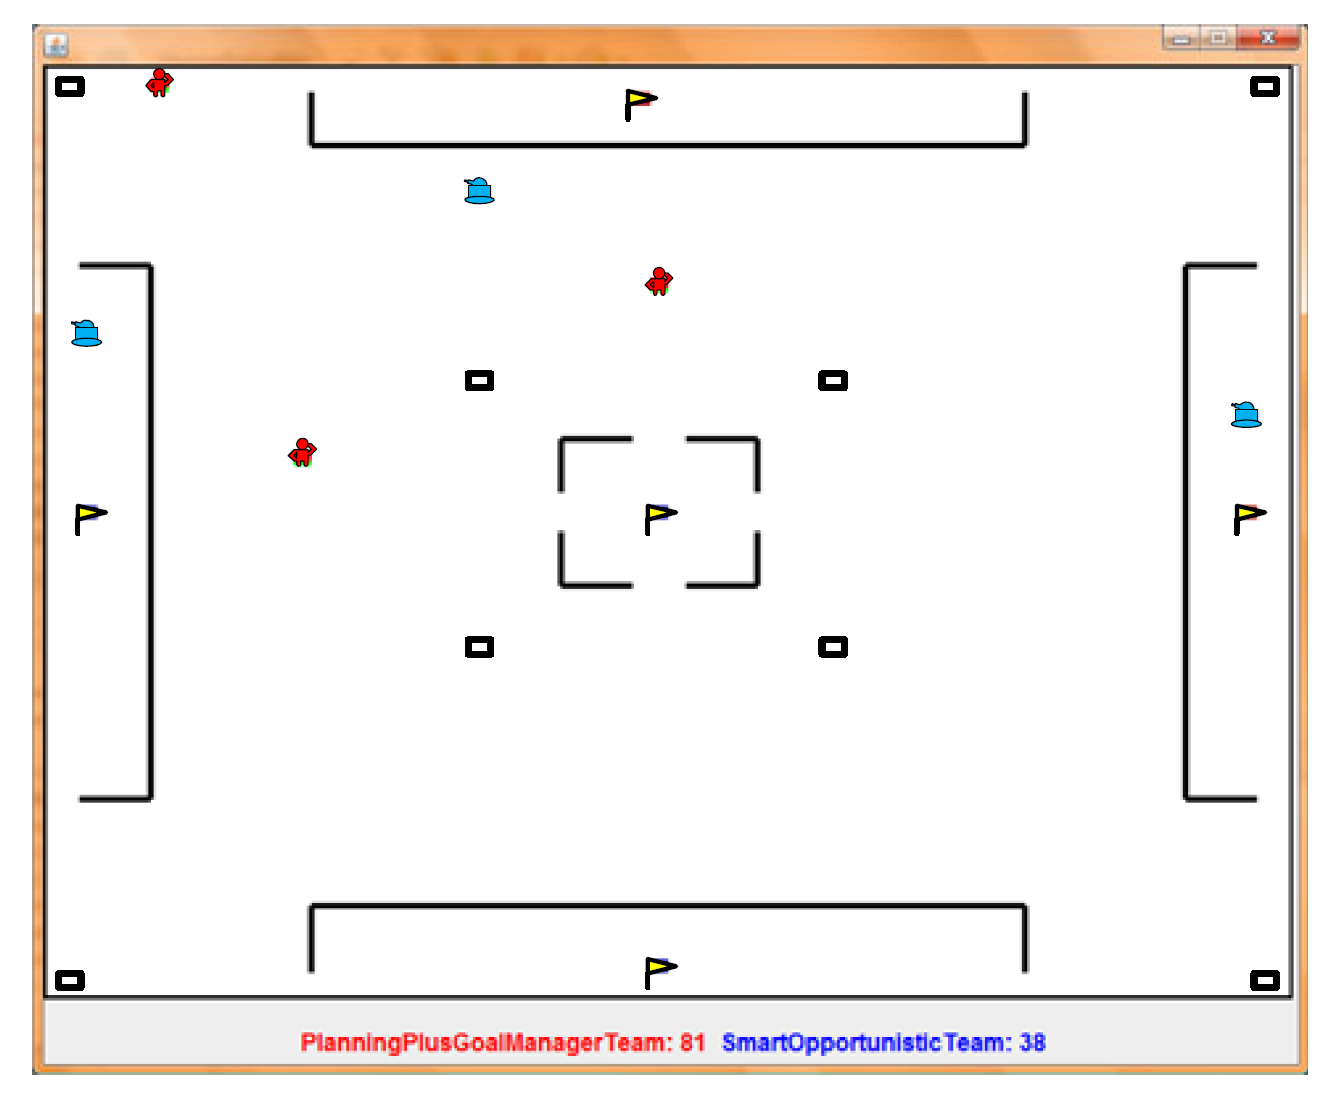
\includegraphics[width=0.27\textwidth]{task1.png}
			\hspace*{30pt}
			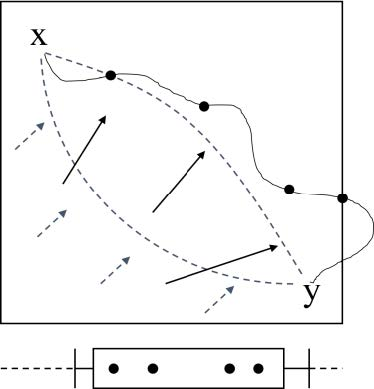
\includegraphics[width=0.2\textwidth]{task2.jpg}
			
		\end{center}
		\begin{itemize}
			\item Задача овладения командным пунктом
			
			\item Задача перемещения в среде с возмущениями
			
			\item Управление подводным аппаратом (большая зона покрытия, встреча с другим кораблем).
			\item Управление БПЛА в военной операции (уменьшение нагрузки на пилота, охрана места крушения).
			\item Коллаборативное зондирование в чрезвычайных ситуациях (оценка состояние среды и нахождение пострадавших, разгрузка спасателей).
		\end{itemize}	
	\end{frame}	

	\begin{frame}
		\frametitle{Каузальная матрица}                             
		\centering
		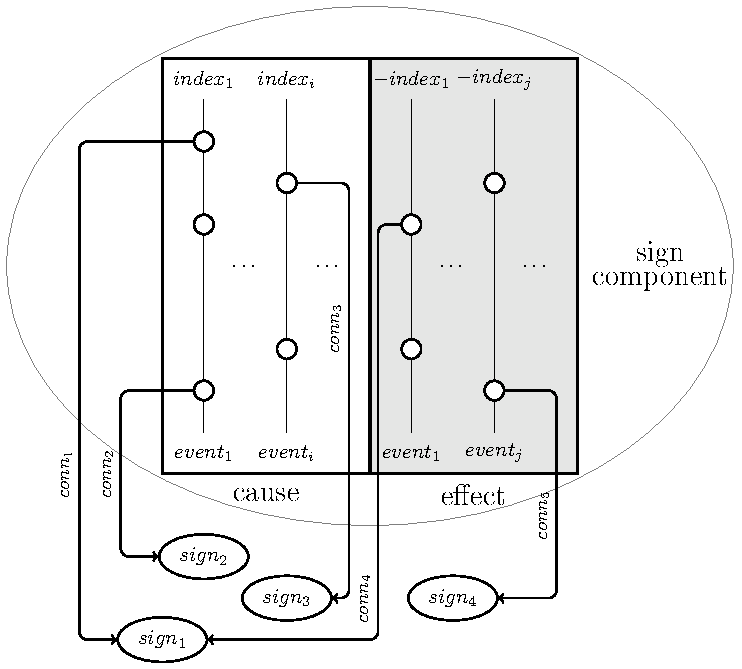
\includegraphics[width=0.7\textwidth]{causnet/caus_matr}
	\end{frame}	

	\begin{frame}
\frametitle{Каузальная сеть на образах}
\footnotesize
\textbf{Каузальная сеть} на множестве образов знаков $W_p=\langle V_p, E_p \rangle$ - помеченный ориентированный граф, в котором
\begin{itemize}
	\item каждому узлу $v\in V_p$ ставится в соответствие кортеж казуальных матриц $Z^p(s)$ образа некоторого знака $s$ ($v\rightarrow Z^p(s)$);
	\item ребро $e=(v_1, v_2)$ принадлежит множеству ребер графа $E$, если $v_1\rightarrow Z^p(s_1), v_2\rightarrow Z^p(s_2)$ и $s_1\in S_p(s_2)$;
	\item каждому ребру графа $e=(v_1, v_2), v_1\rightarrow Z^p(s_1), v_2\rightarrow Z^p(s_2)$ ставится в соответствие метка $\epsilon=(\epsilon_1,\epsilon_2,\epsilon_3)$ - кортеж трех натуральных чисел:
	\begin{itemize}
		\item $\epsilon_1$ - индекс исходной матрицы в кортеже $Z^p(s_1)$, может принимать специальное значение 0, если исходными могут служить любые матрицы из кортежа;
		\item $\epsilon_2$ - индекс целевой матрицы в кортеже $Z^p(s_2)$, строка которой ставится в соответствие признаку $s_1$;
		\item $\epsilon_2$ - индекс столбца в целевой матрице, в которой в соответствующей признаку $s_1$ строке стоит 1, может принимать положительные значения (\textit{столбцы условий}) и отрицательные (\textit{столбцы эффектов}).
	\end{itemize}		
\end{itemize}
\end{frame}

	\begin{frame}
		\frametitle{Каузальная сеть на образах: пример}
	
		\centering
		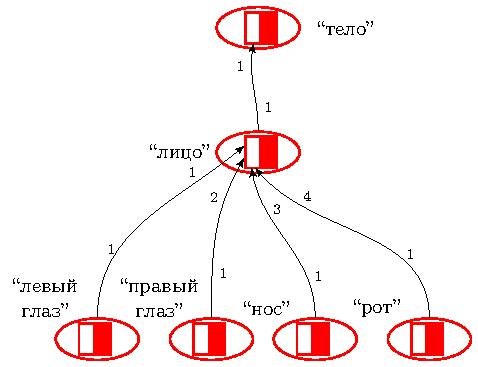
\includegraphics[page=1,width=0.6\textwidth]{examples/causnet/caus_net_colored}
		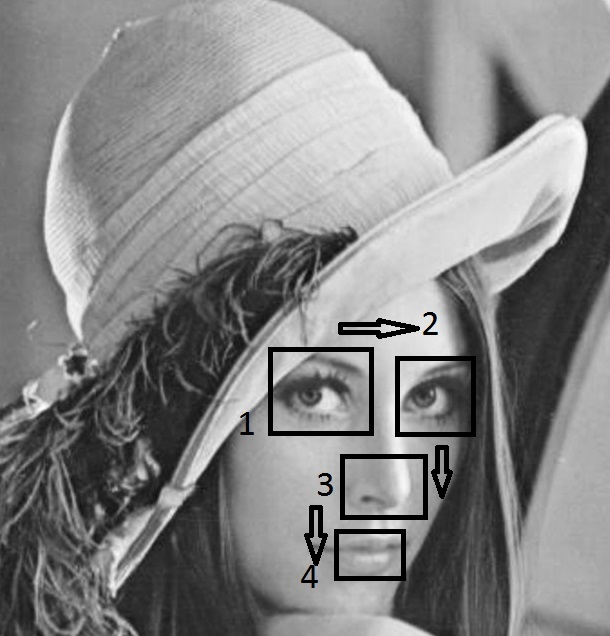
\includegraphics[width=0.4\textwidth]{misc/photos/face}
	\end{frame}
	
	\begin{frame}
		\frametitle{Каузальная сеть на значениях: пример}
		
		\begin{figure}
		\includegraphics[page=2,width=0.7\textwidth]{examples/causnet/caus_net_colored}
		\end{figure}
	
	\end{frame}
	
	\begin{frame}
		\frametitle{Каузальная сеть на личностных смыслах: пример}
		
		\begin{figure}
		\includegraphics[page=3,width=0.7\textwidth]{examples/causnet/caus_net_colored}
		\end{figure}
	
	\end{frame}		

	\begin{frame}
		\frametitle{Планирование в КМ}
		
		\begin{figure}
			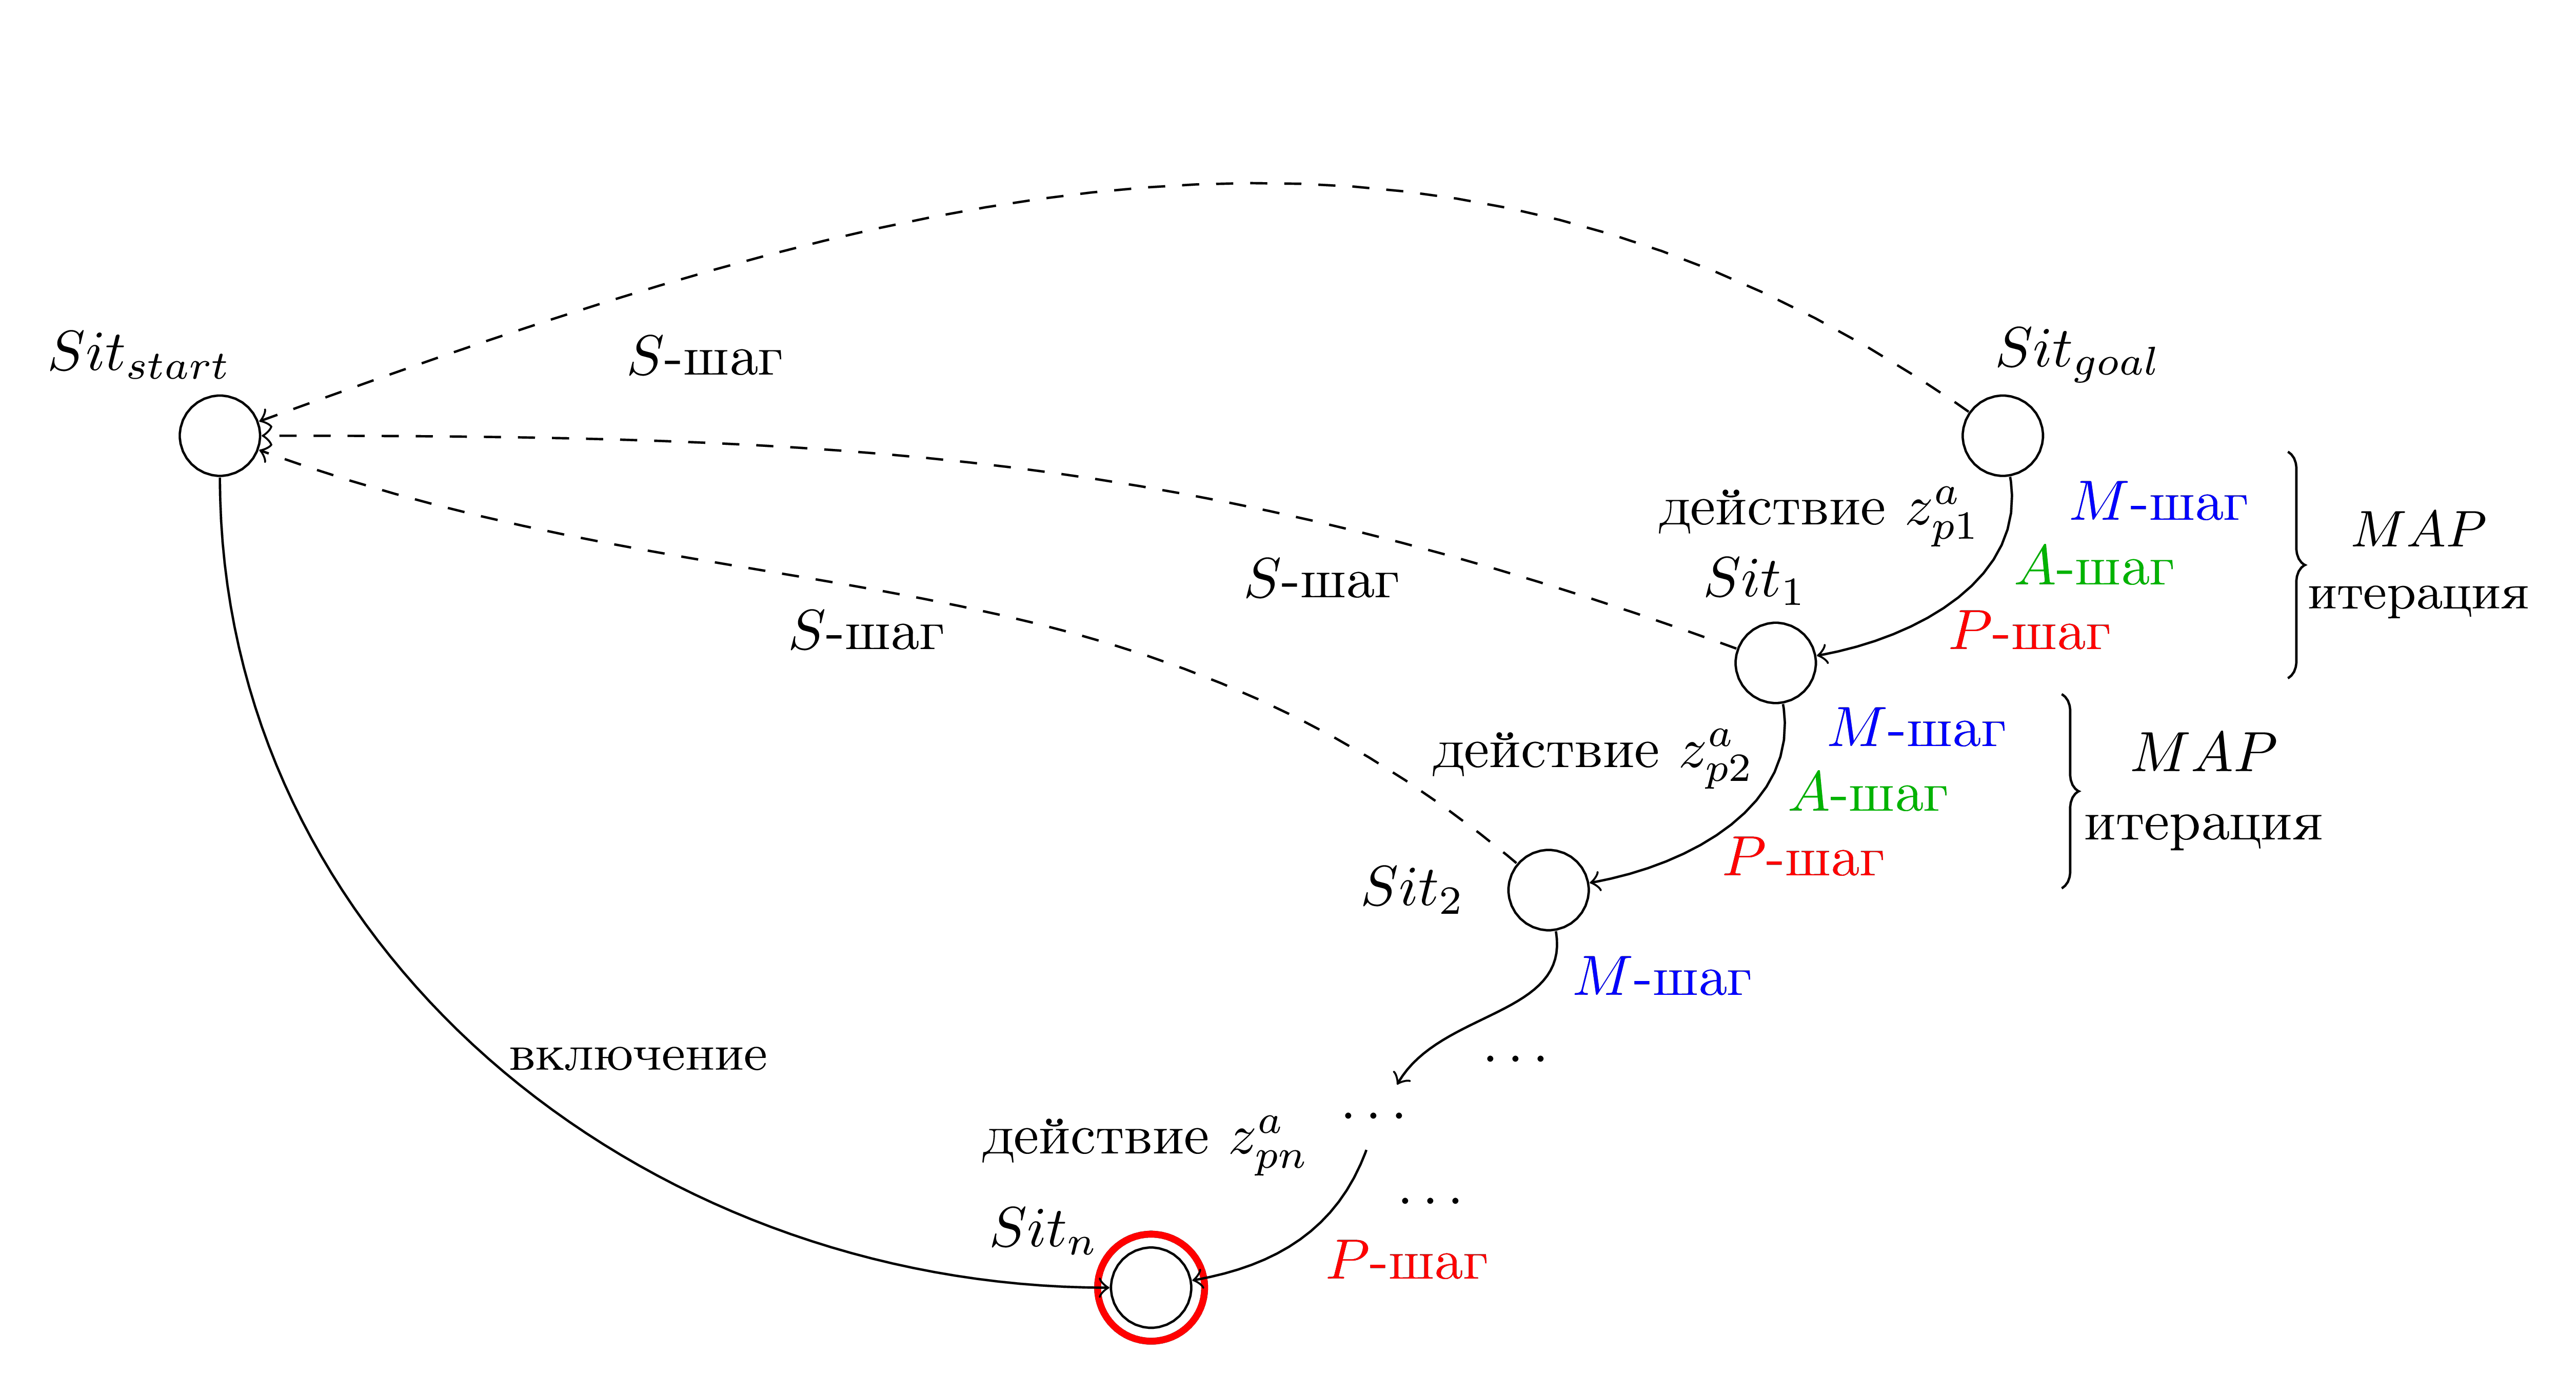
\includegraphics[width=\textwidth]{algo/ru/map_ru}
		\end{figure}
		
	\end{frame}	

	\begin{frame}
		\frametitle{Целеполагание в КМ}
		
		\begin{figure}
			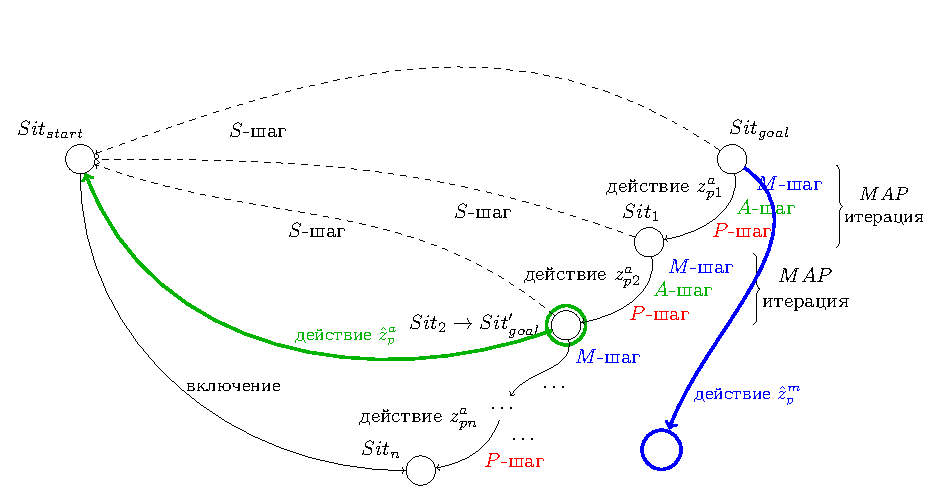
\includegraphics[width=0.8\textwidth]{algo/ru/gmap_ru}
		\end{figure}
		<<Внутреннее>> целеполагание - нахождение схематического действия $\hat z_p^a$ на сети личностных смыслов.
		
		<<Внешнее>> целеполагание - нахождение конкретизированного действия $\hat z_p^m$ в известных сценариях на сети значений.
	\end{frame}								
%	\begin{frame}
%		\frametitle{Цели курса}
%		
%		\begin{columns}
%			\begin{column}{0.5\textwidth}
%				
%			\end{column}
%			\begin{column}{0.5\textwidth}
%				\begin{figure}
%					
\includegraphics[width=\textwidth]{logo}
%				\end{figure}
%			\end{column}
%		\end{columns}
%	\end{frame}
	%	\begin{frame}
	%		\frametitle{Цели курса}
	%		
	%		\begin{itemize}
	%			\item
	%		\end{itemize}
	%	\end{frame}
	
\end{document}
	
	
